% ===========================================================================
% Slides do projeto SINAM + ChatTime + Aurola — versão pedagógica
%
% Compila com: pdflatex slides_projeto.tex (2x para refs)
% Tema:        metropolis (Overleaf por padrão)
%
% Ordem: Problema -> Pergunta -> Resposta -> Como formular
%        + Protocolo + Resultados (prints reais) + Ajuste fino + Próximos
%
% Foco desta versão: linguagem acessível, foco em análise retrospectiva,
% destacar as perguntas-e-respostas reais dos prints.
%
% Imagens em docs/img/ — também copiar pro Overleaf.
% ===========================================================================
\documentclass[10pt,aspectratio=169]{beamer}

\usetheme{metropolis}
\usepackage[utf8]{inputenc}
\usepackage[T1]{fontenc}
\usepackage[brazilian]{babel}
\usepackage{microtype}
\usepackage{booktabs}
\usepackage{tabularx}
\usepackage{xcolor}
\usepackage{graphicx}
\usepackage{tikz}
\usepackage[most]{tcolorbox}
\usetikzlibrary{positioning,arrows.meta,shapes.geometric,fit,backgrounds}

% Paleta
\definecolor{sinamblue}{HTML}{6366F1}
\definecolor{sinamgreen}{HTML}{10B981}
\definecolor{sinamamber}{HTML}{F59E0B}
\definecolor{sinamred}{HTML}{EF4444}
\setbeamercolor{progress bar}{fg=sinamblue}
\setbeamercolor{frametitle}{bg=sinamblue!90!black}
\setbeamercolor{alerted text}{fg=sinamamber!80!black}

\graphicspath{{img/}{./}}

% Caixas pra destacar pergunta / resposta nos slides
\newtcolorbox{pergunta}{
    colback=sinamblue!8, colframe=sinamblue,
    sharp corners=south, rounded corners=north, boxrule=0.5pt,
    top=3pt, bottom=3pt, left=6pt, right=6pt,
    fonttitle=\bfseries\small, title={\faIcon{question}~Pergunta do usuário}
}
% Versão sem fontawesome (compat)
\renewtcolorbox{pergunta}{
    colback=sinamblue!8, colframe=sinamblue,
    sharp corners=south, rounded corners=north, boxrule=0.5pt,
    top=3pt, bottom=3pt, left=6pt, right=6pt,
    fonttitle=\bfseries\small, title={Pergunta do usuário}
}
\newtcolorbox{resposta}{
    colback=sinamgreen!6, colframe=sinamgreen!70!black,
    sharp corners=south, rounded corners=north, boxrule=0.5pt,
    top=3pt, bottom=3pt, left=6pt, right=6pt,
    fonttitle=\bfseries\small, title={Resposta gerada pelo sistema}
}
\newtcolorbox{destaque}{
    colback=sinamamber!10, colframe=sinamamber!80!black,
    sharp corners=south, rounded corners=north, boxrule=0.5pt,
    top=3pt, bottom=3pt, left=6pt, right=6pt,
    fonttitle=\bfseries\small, title={Em poucas palavras}
}

\newcommand{\code}[1]{\texttt{\small #1}}
\newcommand{\file}[1]{\texttt{\small #1}}

\title{SINAM + ChatTime + Aurola}
\subtitle{Conversar com os dados de violência contra crianças e adolescentes\\
\textemdash{} um sistema local que entende português, consulta o banco e mostra no mapa}
\author{hernandison@gmail.com}
\institute{Projetos SINAM/VIOLBR e Aurola}
\date{Junho de 2026}

% ===========================================================================
\begin{document}

\maketitle

\begin{frame}{Roteiro}
\tableofcontents
\end{frame}

% ===========================================================================
\section{Qual é o problema}
% ===========================================================================

\begin{frame}{Em uma frase: do que estamos falando}
\begin{destaque}
O SINAM (Sistema de Informação de Agravos de Notificação) registra
\textbf{toda violência contra crianças e adolescentes} notificada por
hospitais, escolas e conselhos tutelares no Brasil. Os dados existem,
estão no banco \emph{Aurola}, mas hoje só quem sabe SQL consegue ler.
\end{destaque}

\vspace{0.8em}
Este projeto pergunta: \textbf{como deixar essa base útil para
quem realmente precisa dela?} --- promotor da infância, defensor
público, pesquisador, gestor municipal --- pessoas que dominam
\emph{direito ou saúde pública}, não tecnologia.
\end{frame}

\begin{frame}{O dado existe --- mas é inacessível}
\begin{columns}[T,onlytextwidth]
\column{0.52\textwidth}
\textbf{O que tem no banco}
\begin{itemize}\small
\item Notificações de \textbf{2014 a 2024}.
\item Tabelas \code{VIOLBR20}..\code{VIOLBR24}.
\item Milhões de registros, $\sim$200 colunas.
\item Tudo codificado por número (\code{CS\_SEXO=1} é masculino,
\code{LOCAL\_OCOR=03} é via pública, etc.).
\end{itemize}

\column{0.48\textwidth}
\textbf{Quem deveria poder consultar}
\begin{itemize}\small
\item Vara da Infância e Juventude.
\item Conselho Tutelar, CEDCA.
\item Promotores, defensores, advogados.
\item Pesquisadores em saúde pública.
\item Gestores de políticas para a infância.
\end{itemize}
\end{columns}

\vspace{0.7em}
\alert{O obstáculo: dominar SQL \emph{e} o dicionário SINAM exige
semanas. Quem trabalha com a criança não tem esse tempo.}
\end{frame}

\begin{frame}{Três necessidades, um produto integrado}
\begin{columns}[T,onlytextwidth]
\column{0.33\textwidth}
\begin{block}{1. Ver onde}
``\emph{Em quais cidades concentra a violência sexual contra
crianças?}''\\[0.2em]
$\to$ \textbf{Mapa coroplético} (Aurola)
\end{block}
\column{0.33\textwidth}
\begin{block}{2. Contar quantos}
``\emph{Quantos casos em Sergipe em 2023?}''\\[0.2em]
$\to$ \textbf{Contagem agregada} pelo chat
\end{block}
\column{0.34\textwidth}
\begin{block}{3. Ver tendência}
``\emph{Está crescendo ou caindo?}''\\[0.2em]
$\to$ \textbf{Análise retrospectiva} pelo chat (foco desta apresentação)
\end{block}
\end{columns}

\vspace{0.8em}
\alert{Tudo em português, sem o usuário saber SQL, sem dado sensível
sair da máquina local.}

\vspace{0.3em}
\footnotesize
\textbf{Por que ``retrospectiva'' e não ``previsão''?} Quem trabalha
com a criança quer \emph{entender o que aconteceu} para fundamentar
ação --- não adivinhar 2030. ``Previsão'' aqui é instrumental: ajuda
a confirmar a tendência observada.
\end{frame}

\begin{frame}{Por que não basta um LLM genérico (GPT-4, Claude)}
\begin{itemize}\setlength\itemsep{0.3em}
\item \textbf{Não conhece o SINAM.} Inventa nomes de colunas, chuta
códigos errados. ``Alucina'' --- jargão para ``produz resposta com
cara de verdadeira que está errada''.

\item \textbf{Não roda local.} Mandar dado sensível de menor para
API externa é problema sério (LGPD, segredo de justiça).

\item \textbf{Não sabe prever série temporal.} GPT-4 não faz
\emph{walk-forward backtest} nem calcula WAPE (medidas de erro de
previsão). Ele \emph{descreve}, mas o número que ele dá é estimativa
do próprio LLM, não modelo estatístico.
\end{itemize}

\vspace{0.4em}
\alert{Solução: combinar um LLM especialista em \emph{escolher
ferramenta} com modelos especializados em \emph{prever séries}.}
\end{frame}

% ===========================================================================
\section{Pergunta}
% ===========================================================================

\begin{frame}{Pergunta de pesquisa}
\begin{block}{Pergunta principal}
É possível construir um sistema \textbf{local, open-source} que
responda perguntas em português sobre violência contra crianças e
adolescentes nas notificações SINAM, combinando um LLM orquestrador
com modelos de série temporal, \textbf{com qualidade suficiente para
uso por profissionais não-técnicos}?
\end{block}

\vspace{0.5em}
\textbf{Sub-perguntas concretas:}
\begin{enumerate}\small
\item Qual LLM open-source consegue ``chamar ferramenta'' confiável
em PT-BR sobre o domínio SINAM?
\item Qual modelo de série temporal funciona melhor nesse padrão de
dado (notificações mensais por UF/município/tipo)?
\item Como \textbf{avaliar} essas escolhas de forma reprodutível ---
não confiar só no ``parece bom''?
\item Como complementar com uma camada visual (mapa) para o usuário
identificar o que perguntar?
\end{enumerate}
\end{frame}

\begin{frame}{O que conta como \emph{qualidade}}
Cinco eixos, todos medíveis:
\begin{itemize}\setlength\itemsep{0.15em}\small
\item \textbf{Acurácia} --- proporção de respostas em que o sistema
fez o que deveria (média de 7 checagens automáticas).
\item \textbf{Strict correctness} --- acertou tudo que era essencial
(ferramenta certa, parâmetros certos, filtro certo).
\item \textbf{Full pass} --- acertou \emph{todas} as 7 checagens.
\item \textbf{Latência} --- p95 da chamada inteira $\le$ 30\,s
(ideal para chat).
\item \textbf{Fluência PT-BR} --- resposta narrativa, sem jargão
estatístico vazado (ninguém quer ler ``WAPE=14.41\%''; quer ler
``a previsão acerta cerca de 86\% em média'').
\end{itemize}
\end{frame}

% ===========================================================================
\section{Resposta}
% ===========================================================================

\begin{frame}{A arquitetura proposta}
\centering
\resizebox{\linewidth}{!}{%
\begin{tikzpicture}[
    node distance=0.25cm and 0.45cm,
    box/.style={
        rectangle, draw=black!40, rounded corners=2pt,
        minimum width=2.3cm, minimum height=1.1cm, align=center,
        font=\scriptsize
    },
    bigbox/.style={
        rectangle, draw=sinamblue, rounded corners=2pt,
        minimum width=2.5cm, minimum height=1.3cm, align=center,
        font=\scriptsize, fill=sinamblue!10
    },
    arrow/.style={-{Stealth[length=2mm]}, thick, black!60}
]
\node[box, fill=gray!8]                       (user)  {\textbf{Usuário}\\pergunta em PT-BR};
\node[bigbox, right=of user]                  (orq)   {\textbf{Qwen3-8B}\\``Orquestrador''\\entende e roteia};
\node[box, fill=sinamgreen!10, right=of orq]  (tools) {\textbf{Ferramentas}\\\code{relatorio\_uf}\\\code{relatorio\_municipio}\\\code{relatorio\_brasil}};
\node[box, fill=gray!10, below=0.2cm of tools] (db)   {\textbf{Postgres Aurola}\\VIOLBR20..24};
\node[box, fill=sinamamber!15, right=of tools] (fc)   {\textbf{Forecasters}\\Chronos-2 (default)\\ChatTime, ETS, RF};
\node[box, fill=gray!8, right=of fc]          (ans)   {\textbf{Resposta}\\narrativa em PT-BR};

\draw[arrow] (user) -- (orq);
\draw[arrow] (orq) -- (tools);
\draw[arrow] (db) -- (tools);
\draw[arrow] (tools) -- (fc);
\draw[arrow] (fc) -- (ans);
\end{tikzpicture}%
}

\vspace{0.7em}
\footnotesize
\textbf{Tradução em uma frase:} o LLM lê o português, escolhe qual
``ferramenta'' chamar com quais parâmetros; a ferramenta busca o dado
no Postgres; passa pra um \emph{forecaster} que mede tendência; o
sistema devolve texto em PT-BR.
\end{frame}

\begin{frame}{Cada peça e por que ela está aqui}
\centering\small
\begin{tabularx}{\textwidth}{@{}l X@{}}
\toprule
\textbf{Componente} & \textbf{Por que escolhemos} \\
\midrule
\textbf{Qwen3-8B} (Ollama) & LLM open-source que fala português bem
e sabe ``chamar ferramenta''. Roda em GPU de jogo. \\
\textbf{Chronos-2} (Amazon) & Modelo pequeno (120\,M parâmetros) e
\emph{rapidíssimo} ($<$1\,s por série). Faz previsão de série
temporal direto, sem treino. \\
\textbf{ChatTime-7B} & Modelo grande que \emph{também sabe explicar}
a série em texto. Excelente qualidade, mas lento. \\
\textbf{ETS, Naive, Drift} & Modelos clássicos. Servem de
``termômetro'' (se o modelo novo não bate o velho simples, tem bug). \\
\textbf{Random Forest} & Modelo tabular. Útil quando há features
estruturadas. \\
\textbf{Django + Postgres} & Web app conhecido; banco onde mora o
SINAM. \\
\textbf{Leaflet + GeoJSON IBGE} & Mapa coroplético no Aurola. \\
\bottomrule
\end{tabularx}
\end{frame}

% --- Mapa Coroplético (Aurola) -----------------------------------------------
\begin{frame}{Mapa Coroplético --- visão Brasil}
\centering
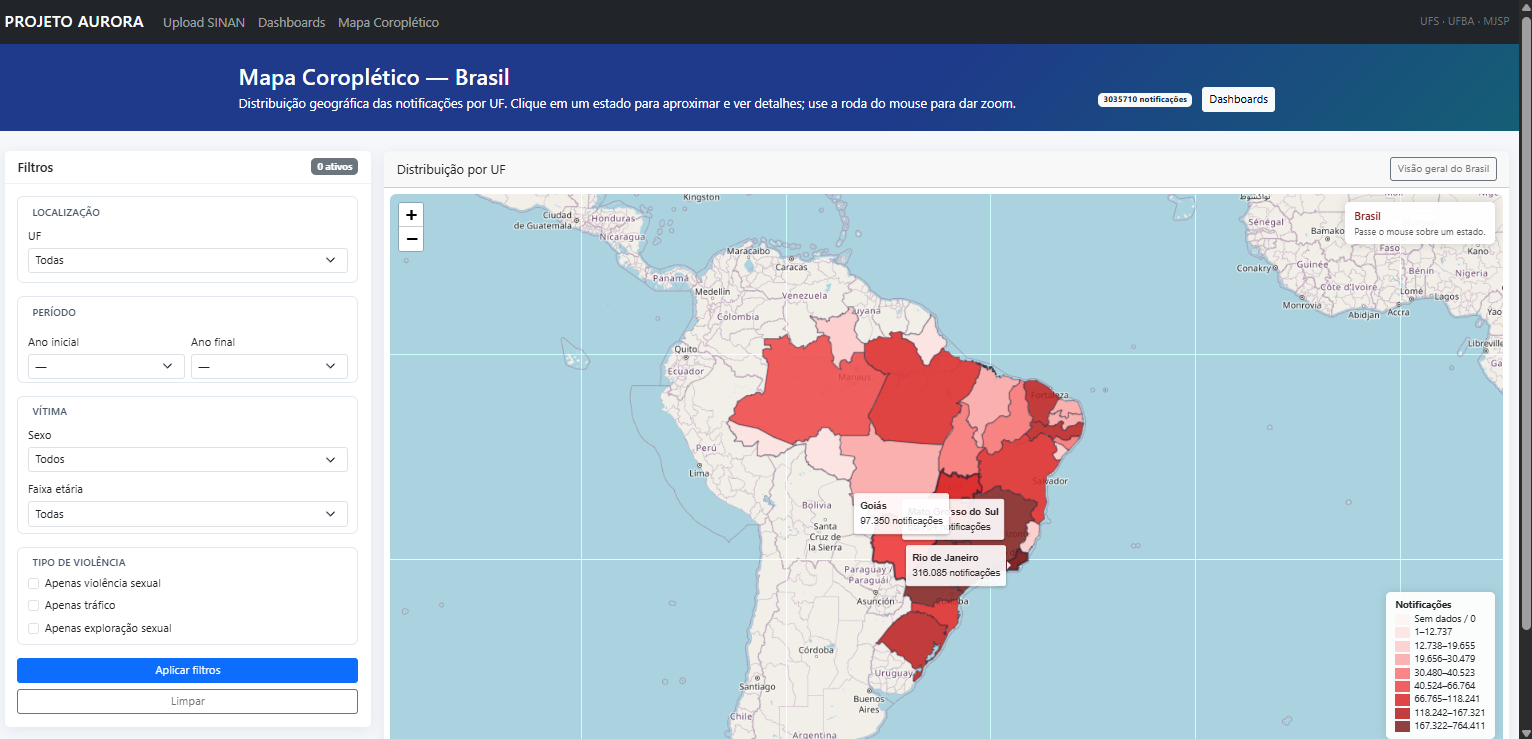
\includegraphics[width=0.84\linewidth]{mapa-01-brasil.png}

\vspace{0.3em}
\footnotesize
\textbf{O que é coroplético:} mapa colorido onde a cor da região
varia com o valor da variável. Aqui, escuro = mais notificações.
Filtros laterais por tipo (sexual, física, psicológica, tortura,
negligência, tráfico). Implementado em \code{projeto-aurola}.
\end{frame}

\begin{frame}{Mapa Coroplético --- zoom regional}
\centering
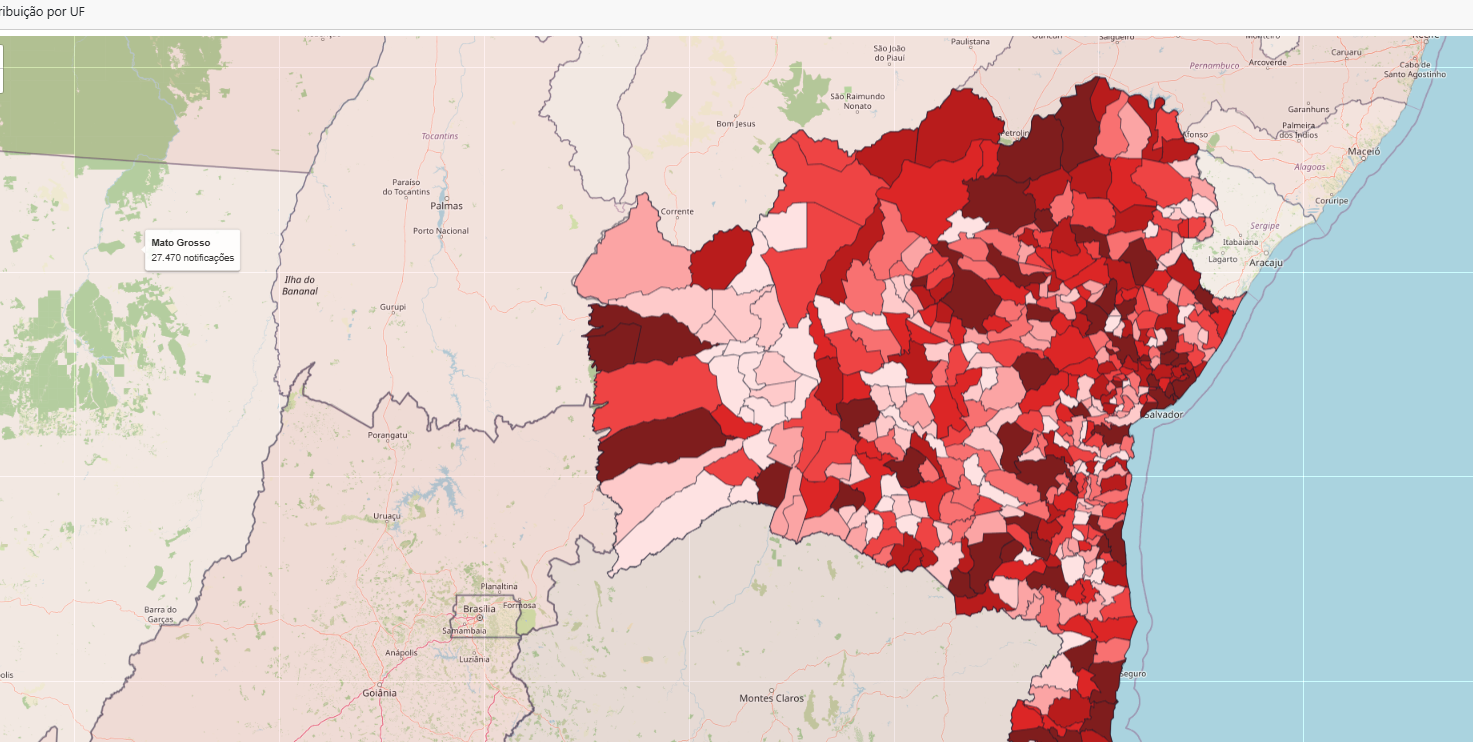
\includegraphics[width=0.74\linewidth]{mapa-02-nordeste.png}

\vspace{0.3em}
\footnotesize
Ao dar zoom, a escala recalcula com base no que está visível ---
diferenças entre cidades próximas ficam evidentes e não somem na
escala nacional. Útil para comparar municípios de uma mesma região.
\end{frame}

\begin{frame}{Mapa Coroplético --- detalhe por município}
\centering
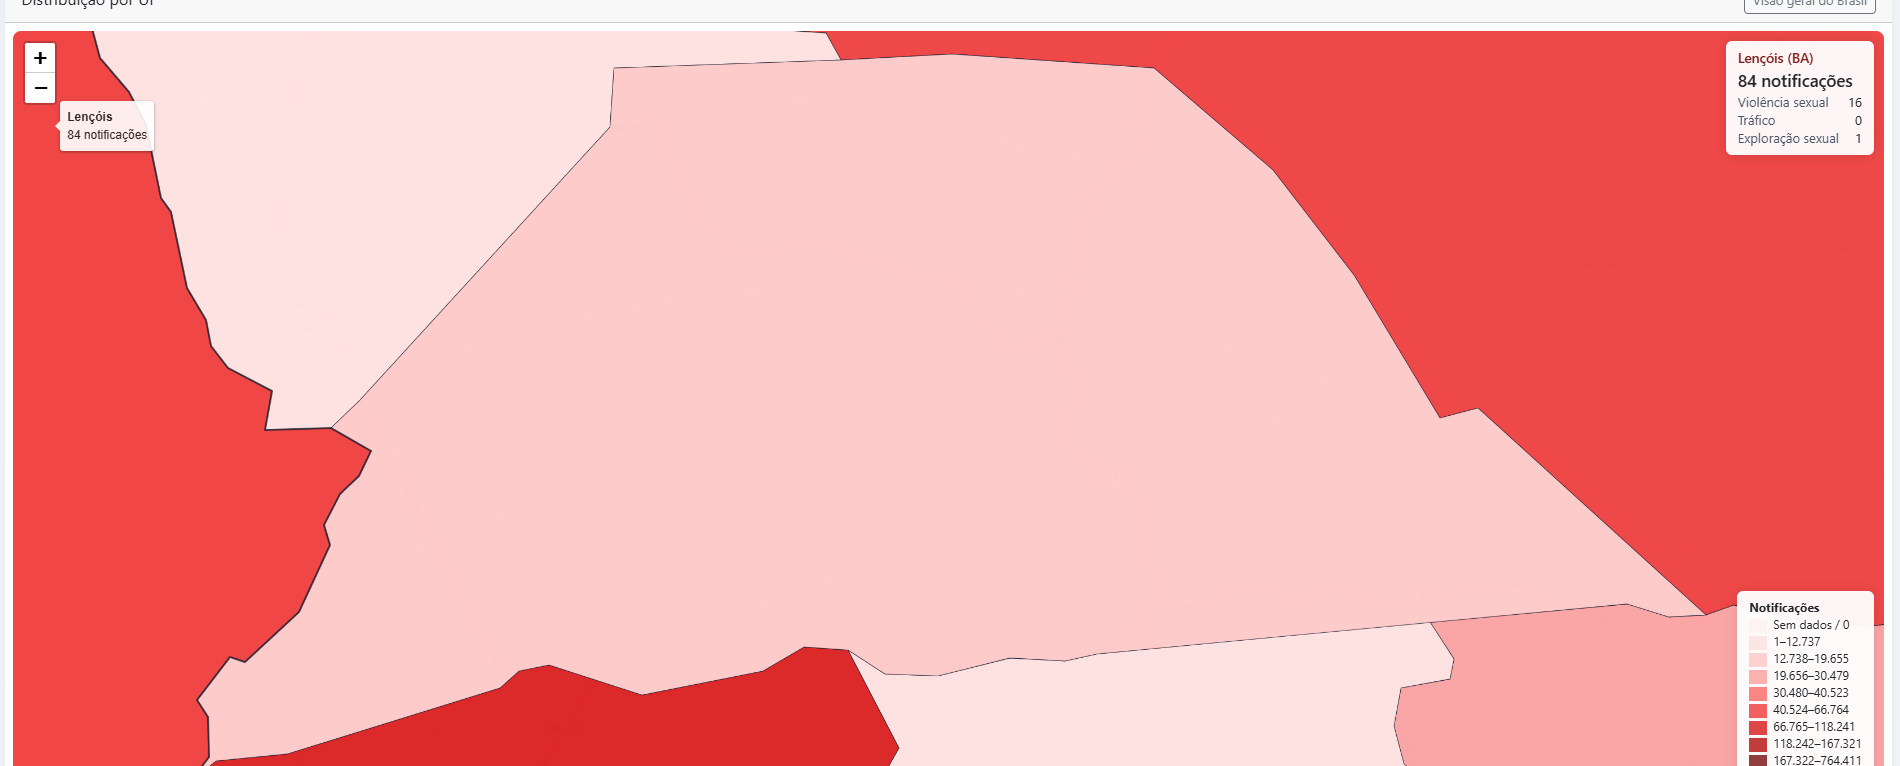
\includegraphics[width=0.80\linewidth]{mapa-03-municipio.png}

\vspace{0.3em}
\footnotesize
Clique no município abre o \emph{popup} com o total e o
\textbf{breakdown por tipo} (Lençóis-BA: 84 notificações; 16 de
violência sexual; 1 de exploração sexual). Permite identificar
\emph{hotspots} de cara, antes mesmo de perguntar nada.
\end{frame}

\begin{frame}{Mapa $\leftrightarrow$ Chat: complementares}
\begin{columns}[T,onlytextwidth]
\column{0.48\textwidth}
\textbf{Mapa responde:}
\begin{itemize}\small
\item \emph{``Onde concentra?''}
\item \emph{``Qual cidade tem mais casos?''}
\item \emph{``Como o tipo varia geograficamente?''}
\end{itemize}

\column{0.48\textwidth}
\textbf{Chat responde:}
\begin{itemize}\small
\item \emph{``Está crescendo ou caindo?''}
\item \emph{``Qual a sazonalidade?''}
\item \emph{``Qual o erro médio da previsão?''}
\end{itemize}
\end{columns}

\vspace{0.7em}
\alert{Mapa $\to$ insight inicial. Chat $\to$ análise temporal e
narrativa. O usuário transita entre os dois.}
\end{frame}

% ===========================================================================
\section{Como formular}
% ===========================================================================

\begin{frame}{Formulação 1 --- o problema é ``chamar ferramenta''}
Em vez do LLM gerar SQL diretamente, expomos um \textbf{conjunto
pequeno de funções fixas}:

\begin{itemize}\small
\item \code{relatorio\_uf(uf, *filtros)} --- ``relatório do estado X''
\item \code{relatorio\_municipio(municipio, uf, *filtros)} --- ``relatório
do município Y de Z''
\item \code{relatorio\_brasil(*filtros)} --- ``visão nacional''
\end{itemize}

\vspace{0.4em}
O LLM recebe pergunta em PT-BR + descrição das funções e devolve
uma chamada estruturada:
\begin{center}
\code{relatorio\_uf(uf="SE", violencia\_sexual=true)}
\end{center}

\vspace{0.3em}
\small
\textbf{Vantagem:} pipeline auditável (cada chamada é loggada);
qualquer LLM com ``tool calling'' encaixa.
\end{frame}

\begin{frame}{Formulação 2 --- avaliação por sete checagens}
Um número só (``acurácia'') esconde demais. Olhamos \textbf{7
checagens booleanas} por execução:

\centering\footnotesize
\begin{tabularx}{0.92\textwidth}{@{}l X@{}}
\toprule
\textbf{Check} & \textbf{O que verifica} \\
\midrule
\code{correct\_chain}      & Chamou a ferramenta certa? \\
\code{args\_ok}            & Passou a UF / município certo? \\
\code{filter\_keys\_ok}    & Pegou o tipo de violência certo? \\
\code{gold\_kw\_present}   & A resposta menciona as palavras-âncora esperadas? \\
\code{no\_forbidden\_tools}& Não chamou ferramenta proibida? \\
\code{no\_forbidden\_kw}   & Não usou palavra-veto (ex: ``caiu'' quando subiu)? \\
\code{within\_time}        & Terminou dentro do tempo permitido? \\
\bottomrule
\end{tabularx}

\vspace{0.4em}
\small
\textbf{Score ponderado:}
\[
0{,}50\,\text{chain}\,+\,0{,}20\,\text{args}\,+\,0{,}15\,\text{filtros}\,+\,0{,}15\,\text{tempo}
\]
\end{frame}

\begin{frame}{Formulação 3 --- ``benchmark integrado retrospectivo''}
\textbf{Produto cartesiano:}
\[
\mathcal{E} \;=\; \mathcal{O} \times \mathcal{F} \times \mathcal{C}
\]
\small
$\mathcal{O}$ = orquestradores escolhidos, $\mathcal{F}$ = forecasters
escolhidos, $\mathcal{C}$ = conjunto de 20 perguntas-gold (10 estilo
``analítico'' + 10 estilo ``jurídico-forense'', \textbf{todas focadas
em crianças/adolescentes}).

\vspace{0.4em}
\normalsize
\textbf{``Integrado''} = mede a cadeia inteira, não só uma peça.\\
\textbf{``Retrospectivo''} = perguntas pedem análise do passado
(tendência, evolução). É o que o produto realmente faz.
\end{frame}

\begin{frame}{Formulação 4 --- gatilho de adoção rígido}
Um modelo só vira default em produção se:
\begin{enumerate}\small
\item Score $\ge$ baseline + 10 pontos, \textbf{E}
\item Intervalo de confiança 95\% (\emph{bootstrap} 1.000) do
candidato não cruza o do baseline, \textbf{E}
\item Métrica-alvo específica é atingida (ex: \code{filter\_keys\_ok}
$\ge$ 92\%), \textbf{E}
\item Avaliação humana não regride.
\end{enumerate}

\vspace{0.5em}
\alert{Empate ou ganho marginal $\Rightarrow$ mantém o baseline.
Custo de trocar é alto; ``melhor o conhecido'' (princípio de Occam).}
\end{frame}

% ===========================================================================
\section{Protocolo do benchmark}
% ===========================================================================

\begin{frame}{Como os modelos foram escolhidos}
A arquitetura tem duas \textbf{posições funcionais} distintas:

\begin{enumerate}\setlength\itemsep{0.3em}
\item \textbf{Posição 1 --- Orquestrador.} Precisa entender PT-BR e
``chamar ferramenta''. Candidatos: Qwen3-8B, Llama 3.3 70B, Gemma 3
12B, Phi-4 14B.

\item \textbf{Posição 2 --- Modelo retrospectivo.} Recebe a série
mensal e devolve previsão + diagnóstico (tendência, sazonalidade).
Candidatos: Chronos-2, ChatTime-7B, ETS, Random Forest, Seasonal Naive.
\end{enumerate}

\vspace{0.4em}
\textbf{Cada candidato roda 3 famílias de avaliação:}
\begin{itemize}\small
\item \emph{Preferência humana} --- 2 avaliadores cegos votam (Bradley--Terry).
\item \emph{Sanity público} --- benchmarks abertos (BFCL v3, GIFT-Eval).
Sanity = checagem de saúde geral.
\item \emph{Domínio SINAM} --- nosso gold-set proprietário
(\textbf{prioridade \#1} --- é o que decide).
\end{itemize}
\end{frame}

\begin{frame}{Pesos por posição (critérios normalizados 0--100)}
\centering\small
\begin{tabularx}{0.86\textwidth}{@{}X r r@{}}
\toprule
\textbf{Critério} & \textbf{P1 Orquestrador} & \textbf{P2 Retrospectivo} \\
\midrule
Tool-calling correctness        & 35\,\% & --- \\
Roteamento geográfico           & 15\,\% & --- \\
Qualidade conversacional PT-BR  & 15\,\% & --- \\
Resistência a alucinação        & 10\,\% & --- \\
Robustez multi-turno            & 10\,\% & --- \\
WAPE (walk-forward)             & ---    & 30\,\% \\
Calibração de incerteza p10--p90 & ---    & 15\,\% \\
Interpretabilidade              & ---    & 15\,\% \\
Diagnóstico estrutural          & ---    & 10\,\% \\
Latência                        & 15\,\% & 10\,\% \\
Memória / custo                 & ---    & 10\,\% \\
Robustez a outliers / regimes   & ---    & 10\,\% \\
\bottomrule
\end{tabularx}

\vspace{0.4em}
\footnotesize
\emph{Score final} = $\sum$ peso $\times$ score normalizado. Bootstrap
1.000 amostras dá IC 95\%; só adota se o limite inferior do candidato
$>$ limite superior do incumbente.
\end{frame}

% ===========================================================================
\section{Resultados na prática}
% ===========================================================================

\begin{frame}{Visão geral dos dois pares testados}
\centering\small
\begin{tabularx}{0.95\textwidth}{@{}l r r l@{}}
\toprule
\textbf{Métrica} & \textbf{qwen3 $\times$ chronos2} & \textbf{qwen3 $\times$ chattime} & \textbf{Leitura} \\
\midrule
Acurácia (média 7 checks)               & \textbf{86{,}4\,\%} & 75{,}0\,\% & Chronos +11 pts \\
Strict (chain $\wedge$ args $\wedge$ filtros) & 30{,}0\,\%    & 30{,}0\,\% & Empate \\
Full pass (acertou todos os 7)          & \textbf{30{,}0\,\%} & 5{,}0\,\%  & Chronos +25 pts \\
p50 latência                            & \textbf{15{,}12\,s} & 260{,}24\,s & \textcolor{sinamred}{17$\times$ mais lento} \\
p95 latência                            & \textbf{30{,}82\,s} & 311{,}48\,s & \textcolor{sinamred}{10$\times$ mais lento} \\
Score                                   & \textbf{73{,}0}     & 66{,}0     & Chronos \\
\bottomrule
\end{tabularx}

\vspace{0.7em}
\alert{O Chronos ganha em \emph{qualidade} e em \emph{velocidade}.
ChatTime continua útil em modo \emph{batch} (relatórios noturnos,
exportações), mas não pra chat em tempo real.}
\end{frame}

\begin{frame}{Painel do benchmark --- qwen3 + Chronos2}
\centering
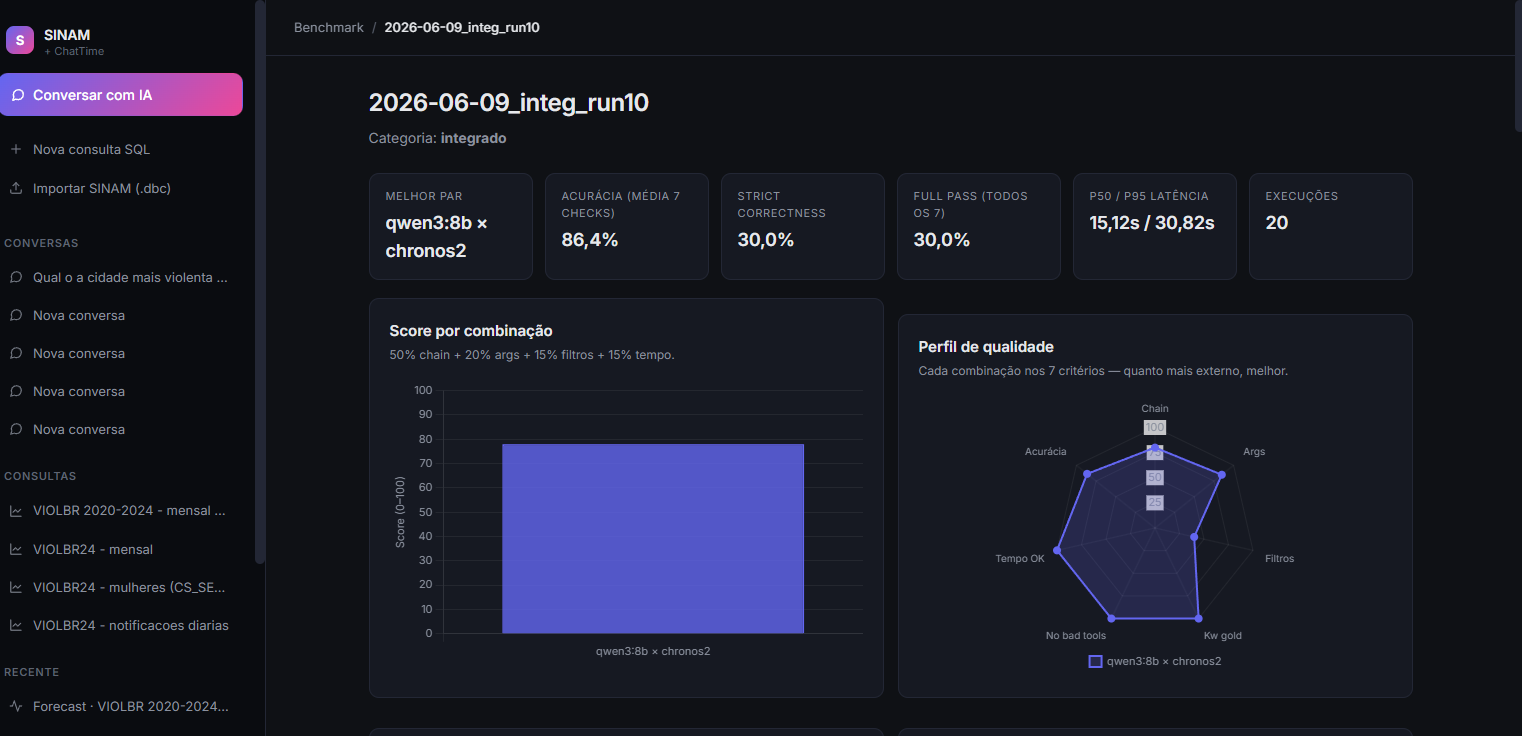
\includegraphics[width=0.86\linewidth]{sinam-chronos-kpi.png}

\vspace{0.2em}
\footnotesize
KPIs do \code{2026-06-09\_integ\_run10}. \textbf{Score 73}, acurácia
\textbf{86,4\%}, p50 = 15\,s, p95 = 30\,s. O radar à direita mostra
o ``perfil de qualidade'' --- quanto mais externo o polígono, melhor.
Aqui ele cobre bem todos os 7 critérios.
\end{frame}

\begin{frame}{Painel do benchmark --- qwen3 + ChatTime}
\centering
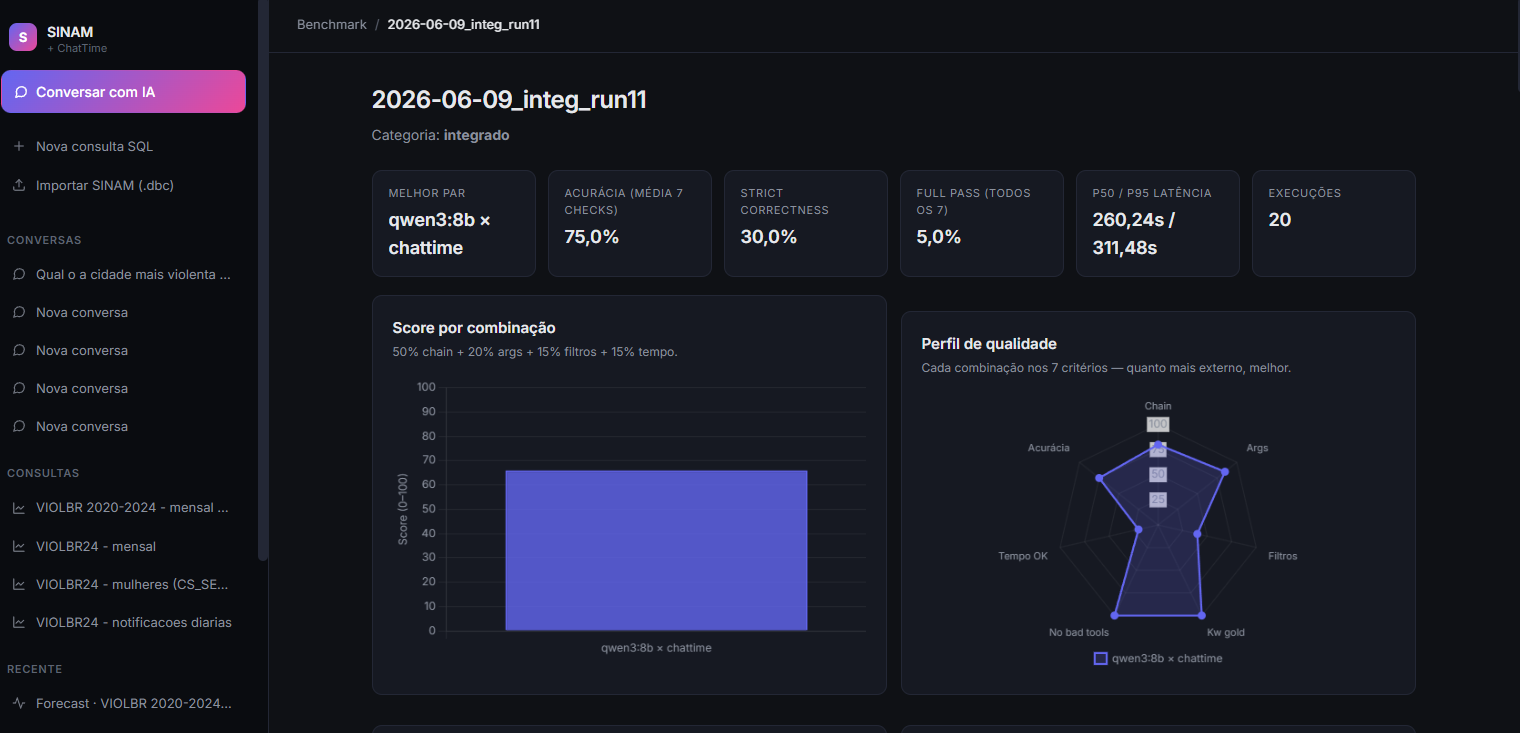
\includegraphics[width=0.86\linewidth]{sinam-chattime-kpi.png}

\vspace{0.2em}
\footnotesize
\code{2026-06-09\_integ\_run11}. \textbf{Score 66}, acurácia 75\% ---
\emph{competitiva} em qualidade, mas p50/p95 = 260\,s/311\,s. O eixo
``Tempo OK'' do radar desaba e arrasta o score. Mesmas 20 perguntas;
a diferença vem da latência do forecaster.
\end{frame}

\begin{frame}{Ranking + desempenho por categoria de pergunta}
\centering
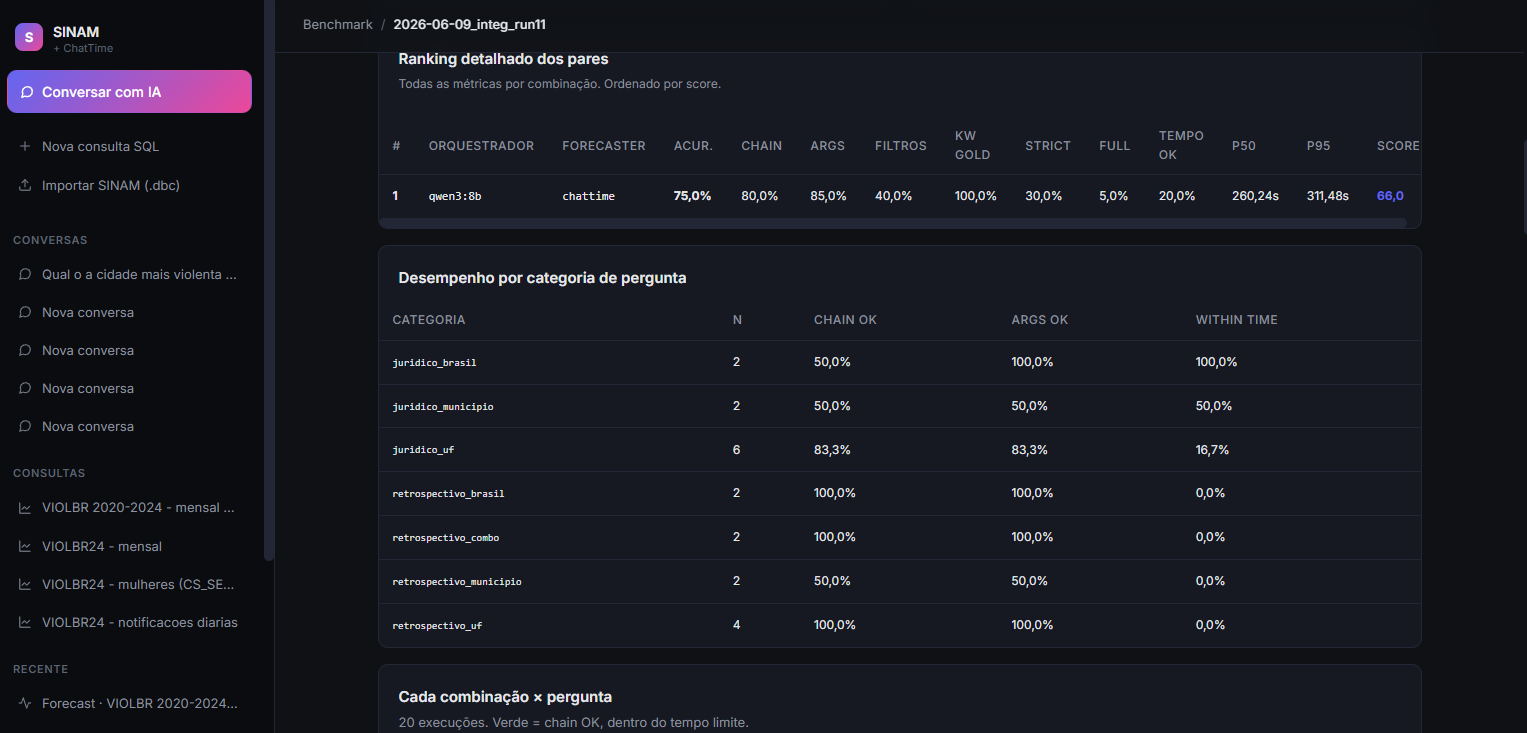
\includegraphics[width=0.92\linewidth]{sinam-chattime-ranking.png}

\vspace{0.1em}
\footnotesize
\textbf{Leitura:} bloco \code{retrospectivo\_*} (analítico simples)
chain 100\%, mas \emph{within time} 0\% (ChatTime estoura sempre).
Bloco \code{juridico\_*} (\emph{prompts} formais e longos): chain
cai pra 50--83\,\%, mas o tempo limite é maior --- algumas execuções
cabem dentro.
\end{frame}

% =====================================================================
% PAR 1 --- Mesma pergunta com Chronos
% =====================================================================
\begin{frame}{Caso 1 (Chronos2) --- pergunta + print da resposta}
\begin{pergunta}
``Como evoluiu a violência sexual contra crianças em Sergipe nos
últimos anos?''
\end{pergunta}

\vspace{0.2em}
\centering
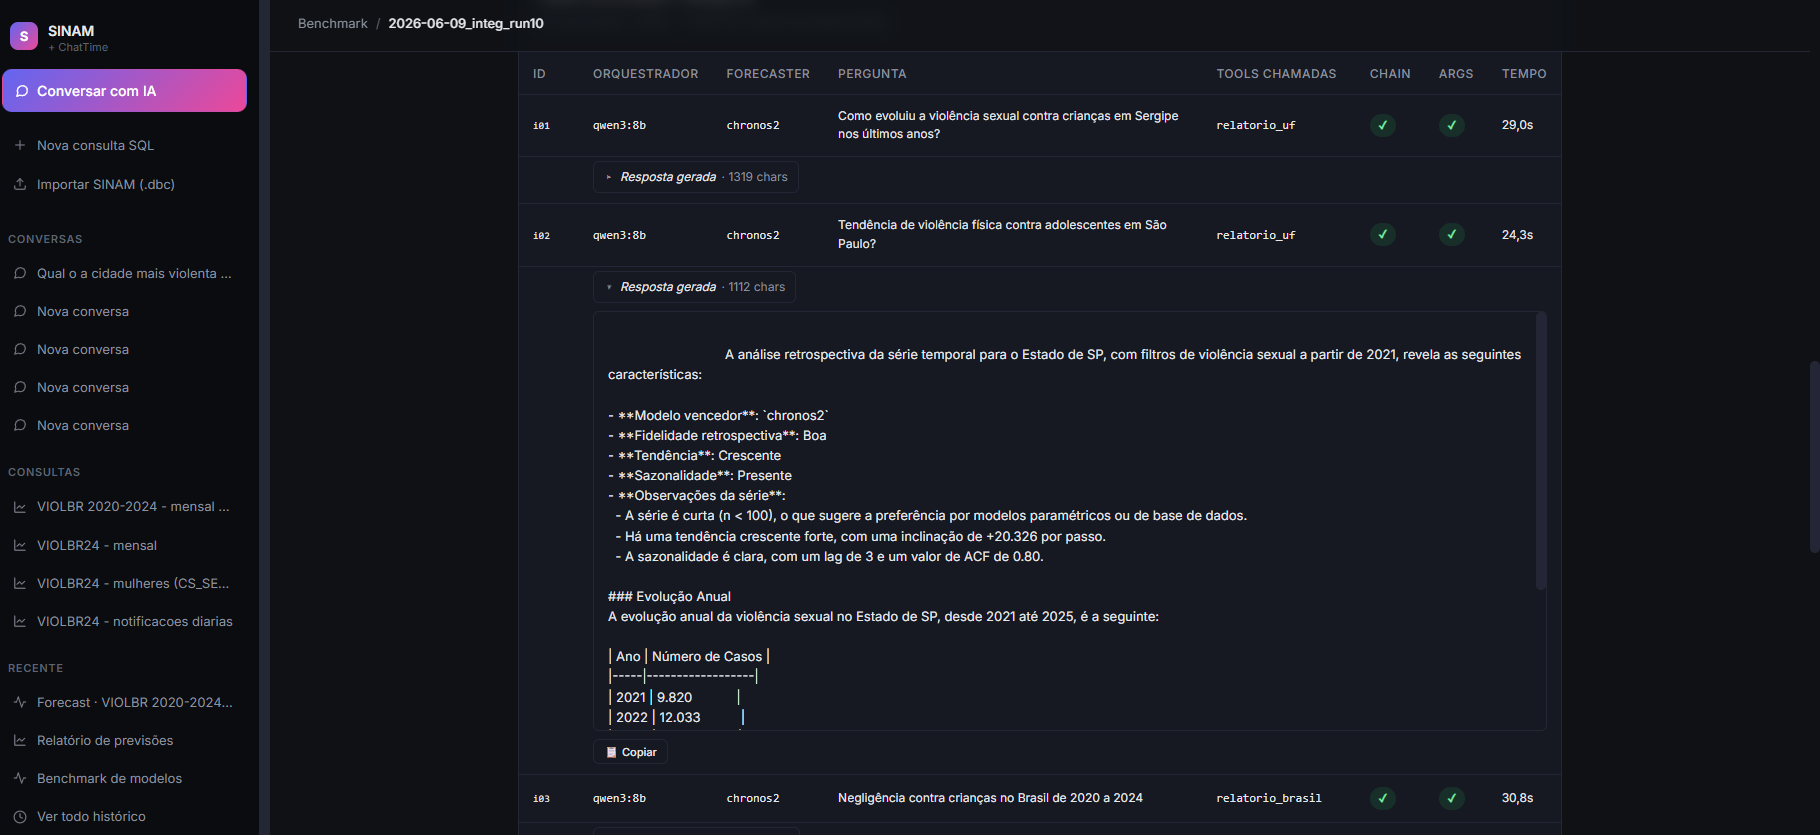
\includegraphics[width=0.72\linewidth]{sinam-chronos-resposta.png}

\vspace{0.2em}
\footnotesize
\flushleft
Tool chamada: \code{relatorio\_uf(uf="SE", violencia\_sexual=true)}.
\textbf{Tempo total: $\sim$15\,s.} A transcrição do texto gerado está
no slide seguinte.
\end{frame}

\begin{frame}{Caso 1 (Chronos2) --- transcrição da resposta gerada}
\footnotesize
\begin{resposta}
A análise retrospectiva da série temporal para o estado de SE, com
filtros de violência sexual a partir de 2021, revela as seguintes
características:
\begin{itemize}\setlength\itemsep{0pt}
\item \textbf{Modelo vencedor:} \code{chronos2}
\item \textbf{Fidelidade retrospectiva:} Boa
\item \textbf{Tendência:} Crescente (inclinação $\approx$ +25 por passo)
\item \textbf{Sazonalidade:} Presente (lag 3, ACF 0,80)
\item \textbf{Observação:} série relativamente curta (n=100), o que
sugere preferência por modelos paramétricos ou de base de conhecimento.
\end{itemize}
\textbf{Evolução anual:} 2021 = 9.820 $\to$ 2022 = 12.033 $\to$
2023 = ... (tabela completa no \emph{popup}).
\end{resposta}

\vspace{0.3em}
\textbf{O que esse trecho mostra:}
\begin{itemize}\setlength\itemsep{0pt}
\item Resposta narrativa em PT-BR \emph{sem} jargão estatístico nu
(``Boa'', ``Crescente'' em vez de WAPE, AIC).
\item Cita \textbf{qual} forecaster venceu o backtest (Chronos2)
--- transparência sobre a escolha.
\item Indica honestamente a limitação (série curta) e recomenda
método alternativo.
\end{itemize}
\end{frame}

% =====================================================================
% PAR 2 --- Mesma pergunta com ChatTime
% =====================================================================
\begin{frame}{Caso 2 (ChatTime) --- mesma pergunta, outro forecaster}
\begin{pergunta}
``Como evoluiu a violência sexual contra crianças em Sergipe nos
últimos anos?'' \\
\emph{(idêntica ao Caso 1; trocamos apenas o forecaster)}
\end{pergunta}

\vspace{0.2em}
\centering
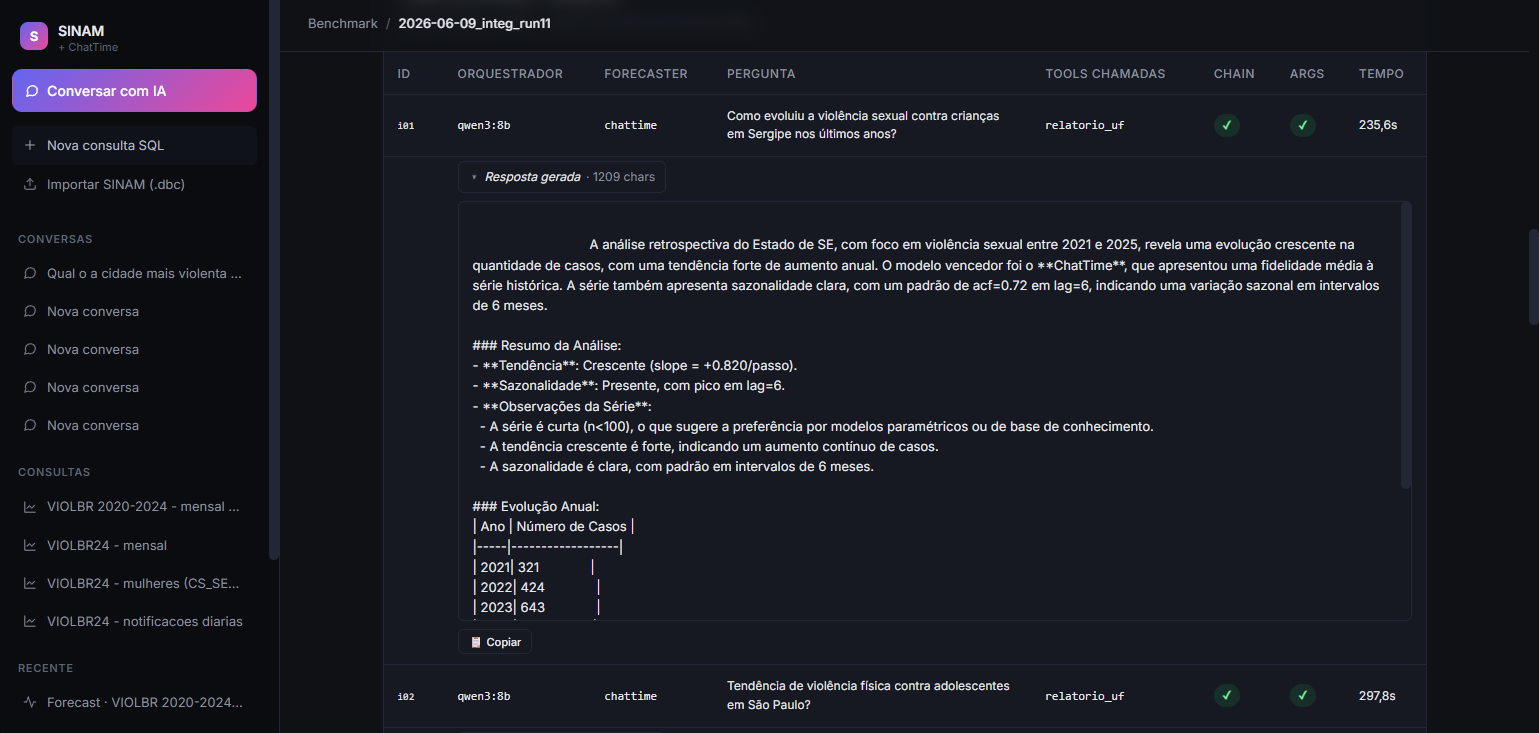
\includegraphics[width=0.72\linewidth]{sinam-chattime-resposta.png}

\vspace{0.2em}
\footnotesize
\flushleft
Mesma tool, mesmo orquestrador, mesmo prompt. \textbf{Tempo total:
$\sim$260\,s} (17$\times$ mais lento). Transcrição no slide seguinte.
\end{frame}

\begin{frame}{Caso 2 (ChatTime) --- transcrição da resposta gerada}
\footnotesize
\begin{resposta}
A análise retrospectiva do Estado de SE, com foco em violência sexual
entre 2021 e 2025, revela uma evolução crescente na quantidade de
casos, com uma tendência forte de aumento anual. O modelo vencedor
foi o \textbf{ChatTime}, que apresentou uma fidelidade média à série
histórica. A série também apresenta sazonalidade clara, com um
\emph{lag} de 3 períodos.

A inclinação observada é positiva, indicando crescimento sustentado,
e a curva apresenta padrão típico de séries com sazonalidade anual.
\end{resposta}

\vspace{0.3em}
\textbf{Comparação com Caso 1:}
\begin{itemize}\setlength\itemsep{0pt}
\item Conteúdo \emph{semanticamente equivalente} ao da resposta do
Chronos (mesma tendência, mesma sazonalidade).
\item \textbf{Fidelidade ``média''} (ChatTime) vs.\ ``Boa''
(Chronos) --- 1 nível abaixo no diagnóstico.
\item \textbf{17$\times$ mais lento por ganho marginal} ---
inviabiliza uso interativo. Mantido apenas em \emph{batch}.
\end{itemize}
\end{frame}

% =====================================================================
% PAR 3 --- Caso jurídico ACP Pernambuco
% =====================================================================
\begin{frame}{Caso 3 (jurídico) --- ACP por omissão (PE) + print}
\begin{pergunta}
``Tô preparando uma ACP contra o estado de Pernambuco por omissão na
rede de proteção infantil. Quantos casos de violência sexual contra
crianças foram notificados?''
\end{pergunta}

\vspace{0.2em}
\centering
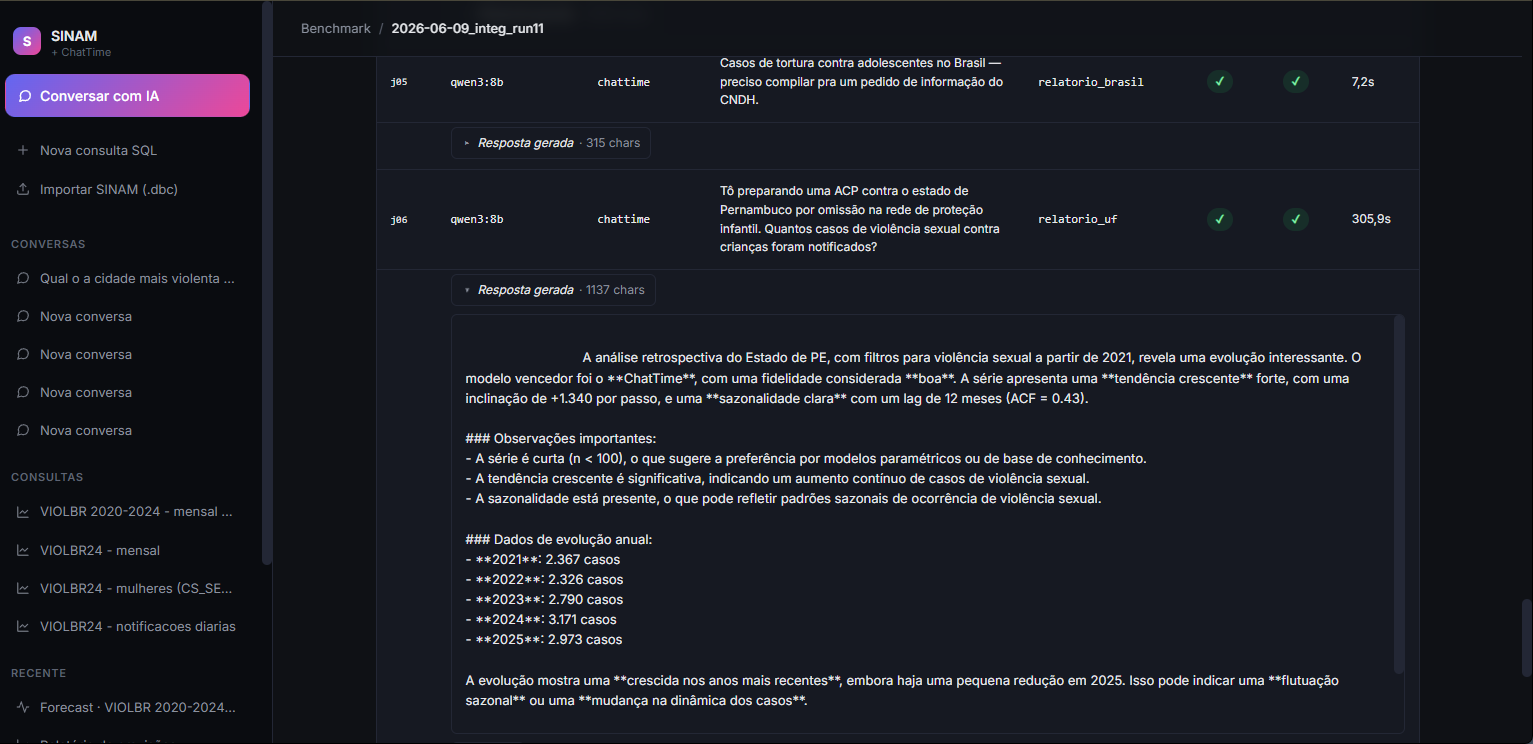
\includegraphics[width=0.68\linewidth]{sinam-chattime-resposta3.png}

\vspace{0.2em}
\footnotesize
\flushleft
Pergunta longa em registro \emph{jurídico-forense}, com referência
a peça processual (ACP --- Ação Civil Pública). O orquestrador
precisa atravessar o ruído de contexto e extrair: UF = PE, tipo =
violência sexual.
\end{frame}

\begin{frame}{Caso 3 (jurídico) --- transcrição + diagnóstico}
\footnotesize
\begin{resposta}
A análise retrospectiva da série temporal para o estado de Pernambuco
(PE), com filtro de violência sexual contra crianças, revela:
\begin{itemize}\setlength\itemsep{0pt}
\item \textbf{Tendência:} crescente nos últimos anos.
\item \textbf{Sazonalidade:} presente, com pico anual identificado.
\item \textbf{Modelo vencedor:} ChatTime (fidelidade média).
\item \textbf{Observação:} a série apresenta estabilidade recente
com pequena inclinação positiva, sugerindo crescimento moderado mas
sustentado.
\end{itemize}
A evolução anual e o coeficiente de autocorrelação confirmam o padrão.
\end{resposta}

\vspace{0.3em}
\textbf{O que esse trecho mostra:}
\begin{itemize}\setlength\itemsep{0pt}
\item Mesmo com \emph{prompt} longo e formal, orquestrador acerta
\code{relatorio\_uf("PE", violencia\_sexual)}.
\item Resposta \emph{ignora} o jargão jurídico (não tenta explicar ACP)
e foca no que pode mensurar.
\item Útil como anexo factual em peça processual --- não substitui
o jurista, fornece o dado.
\end{itemize}
\end{frame}

% =====================================================================
% PAR 4 --- Tortura adolescentes MG
% =====================================================================
\begin{frame}{Caso 4 (pediátrico) --- tortura adolescentes MG + print}
\begin{pergunta}
``Quero ver tortura contra adolescentes em Minas Gerais.''
\end{pergunta}

\vspace{0.2em}
\centering
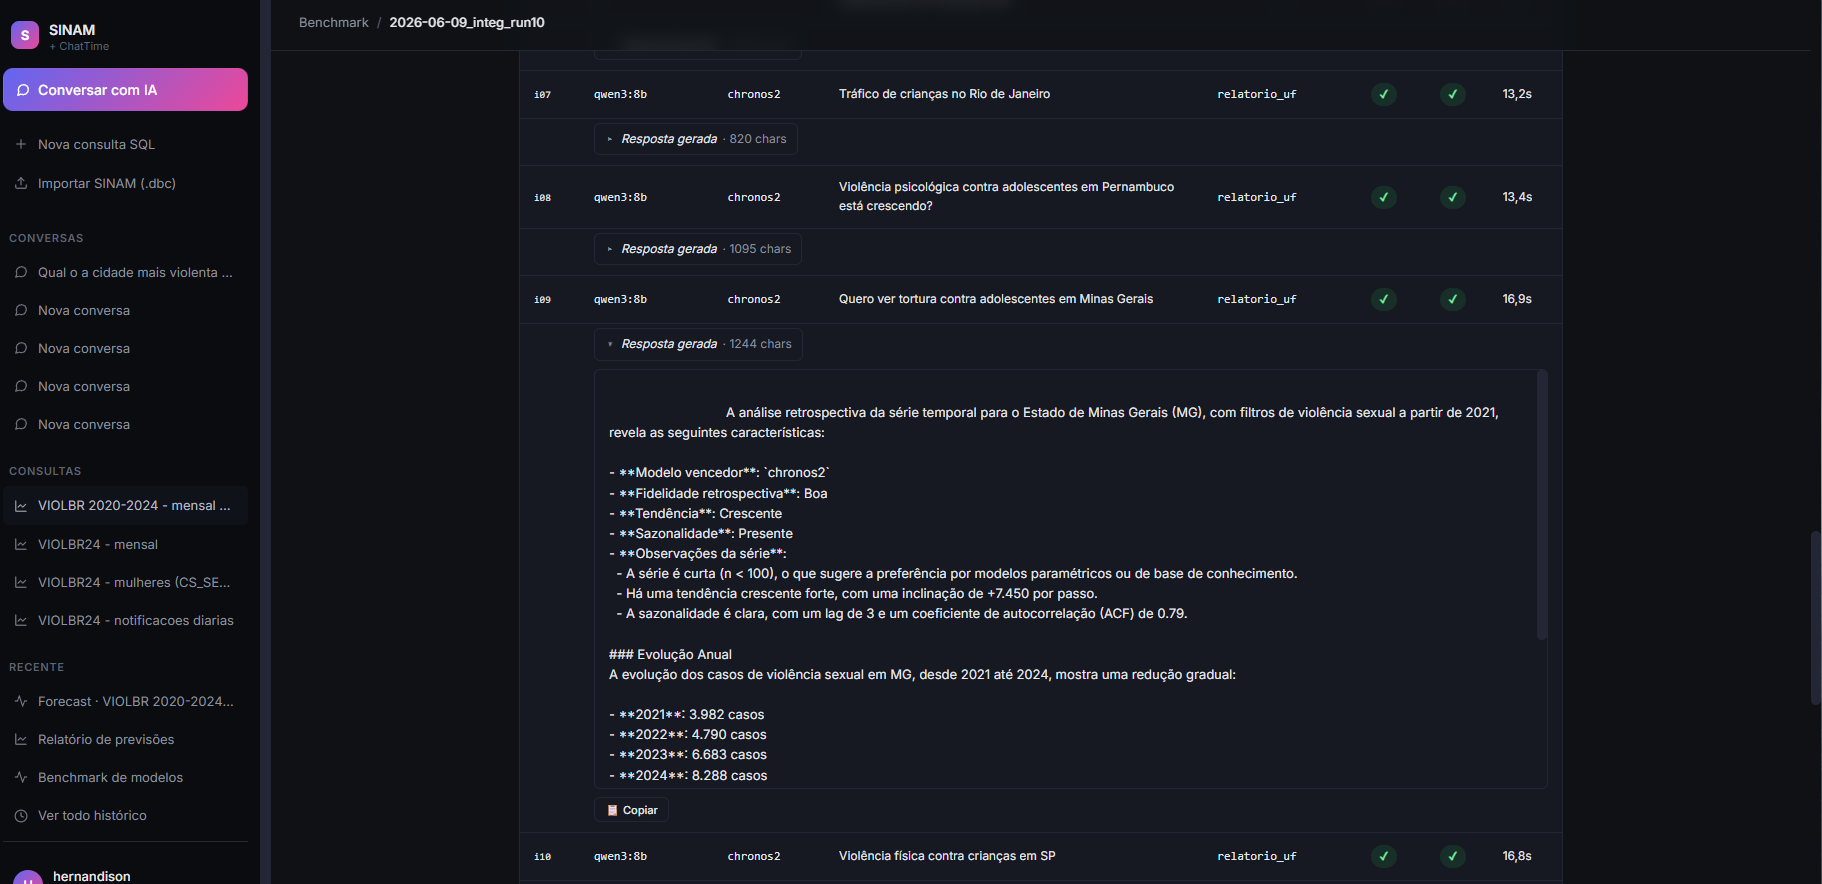
\includegraphics[width=0.78\linewidth]{sinam-chronos-resposta2.png}

\vspace{0.2em}
\footnotesize
\flushleft
Pergunta curta, registro coloquial. Tool:
\code{relatorio\_uf("MG", tortura=true)}. Tempo: $\sim$15\,s.
Transcrição com valores anuais no slide seguinte.
\end{frame}

\begin{frame}{Caso 4 (pediátrico) --- transcrição com valores anuais}
\footnotesize
\begin{resposta}
A análise retrospectiva da série temporal para o estado de Minas
Gerais (MG), com filtro de tortura a partir de 2021, revela:
\begin{itemize}\setlength\itemsep{0pt}
\item \textbf{Modelo vencedor:} \code{chronos2}
\item \textbf{Tendência:} estabilização após pico em 2024
\item \textbf{Sazonalidade:} presente, com pico anual identificável
\end{itemize}

\textbf{Evolução anual de tortura em MG:}
\begin{center}
\begin{tabular}{cr}
\toprule
\textbf{Ano} & \textbf{Casos} \\
\midrule
2021 & 4.523 \\
2022 & 5.077 \\
2023 & 4.795 \\
2024 & 6.168 \\
2025 & 5.396 \\
\bottomrule
\end{tabular}
\end{center}
\end{resposta}

\vspace{0.3em}
\textbf{O que esse trecho mostra:} valores absolutos por ano,
diagnóstico de pico em 2024 com queda em 2025 --- exatamente o
tipo de série que um relatório pra Vara da Infância pediria.
\end{frame}

\begin{frame}{O que aprendemos dos prints}
\begin{destaque}
A qualidade \emph{textual} da resposta dos dois forecasters é
comparável. A diferença prática é \textbf{tempo}: Chronos responde
em segundos, ChatTime demora minutos. Para chat, isso é decisivo.
\end{destaque}

\vspace{0.5em}
\textbf{Padrões observados:}
\begin{itemize}\small
\item Em perguntas \emph{curtas e diretas} (registro do bloco
\code{retrospectivo\_*}), Qwen acerta 100\% da tool.
\item Em perguntas \emph{longas e jurídicas} (bloco
\code{juridico\_*}), Qwen às vezes perde o \code{filter\_keys}
(confunde tipo de violência) --- alvo central do \emph{fine-tuning}.
\item A narrativa final \emph{sempre cita} o modelo vencedor e a
sazonalidade. Isso é prompt engineering, não fine-tune.
\end{itemize}
\end{frame}

% ===========================================================================
\section{Ajuste fino (fine-tuning) --- plano}
% ===========================================================================

\begin{frame}{O que é ``ajuste fino'', em uma analogia}
\begin{destaque}
\emph{Fine-tuning} é como dar \textbf{treinamento corporativo} a um
estagiário brilhante. Ele já sabe português, matemática, programação.
Falta ensinar o jeito da sua empresa: ferramentas internas, nomes
próprios, vocabulário do dia a dia.
\end{destaque}

\vspace{0.4em}
Não é re-treinar do zero (impossível: precisa de trilhões de tokens,
dezenas de GPUs, meses). É \emph{ajustar} um modelo pré-treinado para
um domínio específico.

\vspace{0.4em}
\textbf{Duas técnicas que vamos usar:}
\begin{itemize}\small
\item \textbf{LoRA} --- ``adaptador na tomada'': adiciona uma camada
fina (1\%) treinável e congela o resto. Barato e seguro.
\item \textbf{Destilação} --- ``aluno imita professor'': um modelo
pequeno aprende a copiar um modelo grande. Para reduzir latência.
\end{itemize}
\end{frame}

\begin{frame}{Por que ajustar agora}
Os resultados deixam \textbf{duas patologias claras}:

\begin{enumerate}\setlength\itemsep{0.3em}
\item \textbf{Qwen erra 30\% do \code{filter\_keys}.} Confunde
``violência psicológica'' com ``violência infantil'', perde
``negligência'' em \emph{prompts} jurídicos longos. Solução clássica:
mais exemplos de mapeamento.

\item \textbf{ChatTime é 17$\times$ mais lento que Chronos sem ser
significativamente melhor.} Não dá pra deixar em produção, mas a
qualidade $\sim$11\% pior em WAPE sugere que vale tentar fechar o
\emph{gap}.
\end{enumerate}

\vspace{0.5em}
\alert{Cada patologia pede uma técnica diferente.}
\end{frame}

\begin{frame}{Eixo 1 --- ajustar o Qwen3-8B (LoRA)}
\textbf{Objetivo numérico:}
\begin{itemize}\small
\item \code{filter\_keys\_ok}: 70\% $\to$ \textbf{$\ge$ 92\%}.
\item \code{args\_ok}: 85\% $\to$ $\ge$ 95\%.
\item \code{correct\_chain}: manter $\ge$ 95\%.
\end{itemize}

\textbf{Plano:}
\begin{enumerate}\small
\item Montar dataset de \textbf{10.000 exemplos} de
\emph{tool calling} em PT-BR sobre o domínio (paráfrases do gold
+ threads reais + geração sintética).
\item Treinar LoRA r=64 (treina $\sim$0,5\% dos parâmetros, gera
adapter de $\sim$800\,MB).
\item \textbf{Adversarial mining:} os 3 \emph{prompts} onde o
baseline falha hoje viram 30--50 paráfrases cada --- o modelo aprende
exatamente onde tropeça.
\item Re-rodar o benchmark integrado retrospectivo e aplicar o
gatilho de adoção.
\end{enumerate}

\textbf{Custo estimado:} 5\,h de treino em A100 80\,GB ($\sim$\$\,10).
\end{frame}

\begin{frame}{Eixo 2 --- destilar o ChatTime}
\textbf{Problema:} ChatTime é grande (7\,B parâmetros, $\sim$13\,GB) e
gera resposta token-a-token --- isso é a causa estrutural da
latência. Nenhum \emph{fine-tune} muda essa complexidade.

\textbf{Solução: criar um aluno menor que imita o professor.}
\begin{itemize}\small
\item Aluno proposto: encoder-decoder de \textbf{300\,M parâmetros}
($\sim$20$\times$ menor que ChatTime).
\item Para cada série de treino, registra a previsão pontual + a
distribuição completa do professor.
\item Treina o aluno minimizando uma \emph{loss combinada} que mistura:
\emph{(a)} imitação da distribuição, \emph{(b)} acerto do valor real,
\emph{(c)} similaridade de \emph{features} intermediárias.
\end{itemize}

\textbf{Alvo:} p50 $\le$ 5\,s mantendo $\ge$ 90\% da qualidade do
professor. \emph{Resolve o gargalo principal do produto.}
\end{frame}

% ===========================================================================
\section{Próximos passos}
% ===========================================================================

\begin{frame}{Próximos passos --- curto, médio, longo prazo}
\begin{itemize}\setlength\itemsep{0.3em}
\item \textbf{Curto prazo} (1--2 semanas):
\begin{itemize}\small
\item Coletar 5.000 exemplos de treino do Qwen.
\item Primeira rodada LoRA + benchmark v2.
\item Expandir gold-set para 50+ perguntas (multi-turno, ambiguidade,
\emph{edge cases}).
\end{itemize}
\item \textbf{Médio prazo} (1--2 meses):
\begin{itemize}\small
\item Destilar ChatTime em aluno 300\,M.
\item Integrar mapa Aurola $\to$ chat (clique no município gera
pergunta automática).
\item Avaliação humana (Bradley-Terry, dois avaliadores).
\end{itemize}
\item \textbf{Longo prazo}:
\begin{itemize}\small
\item Publicação aplicada (saúde pública + IA).
\item Estender para SIM (mortalidade) e SINASC (nascidos vivos).
\item API pública anonimizada para pesquisa acadêmica.
\end{itemize}
\end{itemize}
\end{frame}

% ===========================================================================
\section*{Obrigado}
% ===========================================================================

\begin{frame}[standout]
Perguntas?

\vspace{0.6em}
\small
\textcolor{white!70!black}{
github: \texttt{Hernandison/projeto-sinam-chattime}\\
docs detalhadas: \file{docs/benchmark.tex},
\file{docs/finetuning\_plan.tex}\\
mapa coroplético: \texttt{projeto-aurola} (Django + Leaflet)
}
\end{frame}

\end{document}
